\documentclass[12pt, twoside]{book}
%\documentclass[12pt, oneside]{book}  % jednostranna tlac

%spravne nastavenie okrajov
\usepackage[a4paper,top=2.5cm,bottom=2.5cm,left=3.5cm,right=2cm]{geometry}
%zapnutie fontov pre UTF8 kodovanie
\usepackage[utf8]{inputenc}
\usepackage[T1]{fontenc}
\usepackage{amsmath}
\usepackage{enumitem}

%zapnutie slovenskeho delenia slov
%a automatickych nadpisov ako Obsah, Obrázok a pod. v slovencine
%\usepackage[slovak]{babel} % vypnite pre prace v anglictine!

%nastavenie riadkovania podla smernice
\linespread{1.25} % hodnota 1.25 by mala zodpovedat 1.5 riadkovaniu

% balicek na vkladanie zdrojoveho kodu
\usepackage{listings}
% ukazky kodu su cislovane ako Listing 1,2,...
% tu je Listing zmenene na Algoritmus 1,2,...
\renewcommand{\lstlistingname}{Algorithm}
% nastavenia balicka listings
% mozete pridat aj language=...
% na nastavenie najcastejsie pouzivaneho prog. jazyka
% takisto sa da zapnut cislovanie riadkov
\lstset{frame=lines}

% balicek na vkladanie obrazkov
\usepackage{graphicx}
% balicek na vkladanie celych pdf dokumentov, tu zadanie
\usepackage{pdfpages}
% balicek na spravne formatovanie URL
\usepackage{url}
% balicek na hyperlinky v ramci dokumentu
% zrusime farebne ramiky okolo liniek aby pdf
% vyzeralo rovnako ako tlacena verzia
\usepackage[hidelinks,breaklinks]{hyperref}

% -------------------
% --- Definicia zakladnych pojmov
% --- Vyplnte podla vasho zadania, rok ma byt rok odovzdania
% -------------------
\def\mfrok{2024}
\def\mftitle{Analysis, Design and Implementation of Micro-frontend Architecture}
\def\mftyp{Bachelor Thesis}
\def\mfauthor{Bc. Pavol Repiský}
\def\mfskolitel{RNDr. Ľubor Šešera, PhD.}

%ak mate konzultanta, odkomentujte aj jeho meno na titulnom liste
\def\mfkonzultant{Ing. Juraj Marák}  

\def\mfmiestocas{Bratislava, \mfrok}
\def\mfuniverzita{COMENIUS UNIVERSITY IN BRATISLAVA}
\def\mffakulta{FACULTY OF MATHEMATICS PHYSICS AND INFORMATICS}
\def\mftypprace{Diploma thesis}

\def\mfodbor{Computer Science}
\def\program{Applied Computer Science}

% Ak je školiteľ z FMFI, uvádzate katedru školiteľa, zrejme by mala byť aj na zadaní z AIS2
\def\mfpracovisko{Department of Computer Science}

\begin{document}     
\frontmatter
\pagestyle{empty}

\noindent
\begin{minipage}{\textwidth}
    \begin{center}
      \textbf{\mfuniverzita\\
      \mffakulta}
    \end{center}
\end{minipage}

\vfill
\begin{figure}[!hbt]
	\begin{center}
		
\includegraphics[width=0.4\textwidth]{images/FMFI_logo_BP.png}
		\label{img:logo}
	\end{center}
\end{figure}
\begin{center}
		\textbf{\MakeUppercase{\Large\mftitle}}\\
    \mftypprace
\end{center}
\vfill
\mfrok \hfill
\mfauthor
%\eject 
\cleardoublepage
% --- koniec obalky ----



% -------------------
% --- Titulný list
% -------------------
\thispagestyle{empty}
\noindent
\begin{minipage}{\textwidth}
    \begin{center}
      \textbf{\mfuniverzita\\
      \mffakulta}
    \end{center}
\end{minipage}

\vfill
\begin{figure}[!hbt]
    \begin{center}
        
\includegraphics[width=0.4\textwidth]{images/FMFI_logo_BP.png}
        \label{img:logo_dark}
    \end{center}
\end{figure}

\begin{center}
	\textbf{\MakeUppercase{\Large\mftitle}}\\
	\mftypprace
\end{center}
\vfill


\begin{tabular}{l l}
Study program: & \program \\
Branch of study: & \mfodbor \\
Department: & \mfpracovisko \\
Supervisor: & \mfskolitel \\
Consultant: & \mfkonzultant \\
\end{tabular}

\vfill
\noindent
\mfmiestocas \hfill
\mfauthor
%\eject 
\cleardoublepage
% --- Koniec titulnej strany



% -------------------
% --- Zadanie z AIS
% -------------------
% v tlačenej verzii s podpismi zainteresovaných osôb.
% v elektronickej verzii sa zverejňuje zadanie bez podpisov
% v pracach v anglictine anglicke aj slovenske zadanie

\newpage
\setcounter{page}{2}
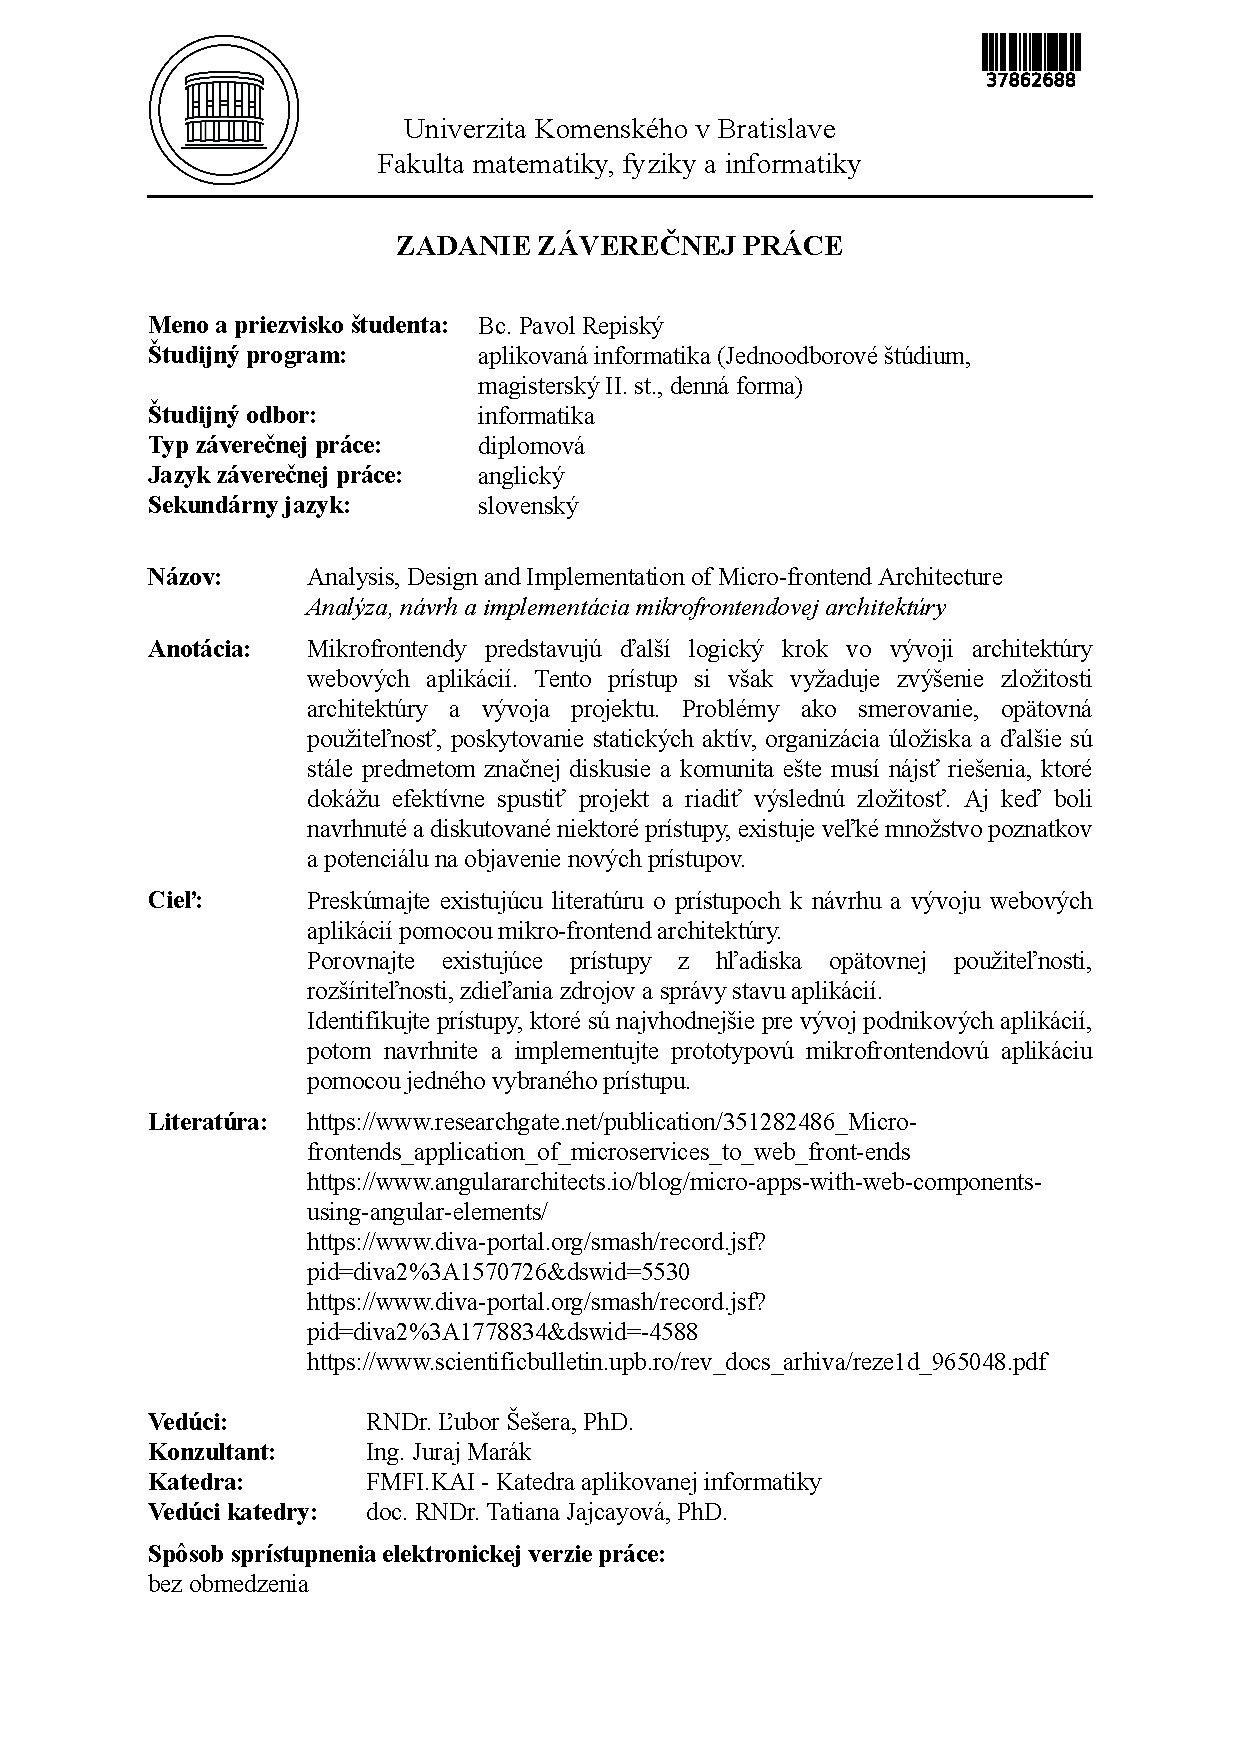
\includepdf{images/zadanie.pdf}
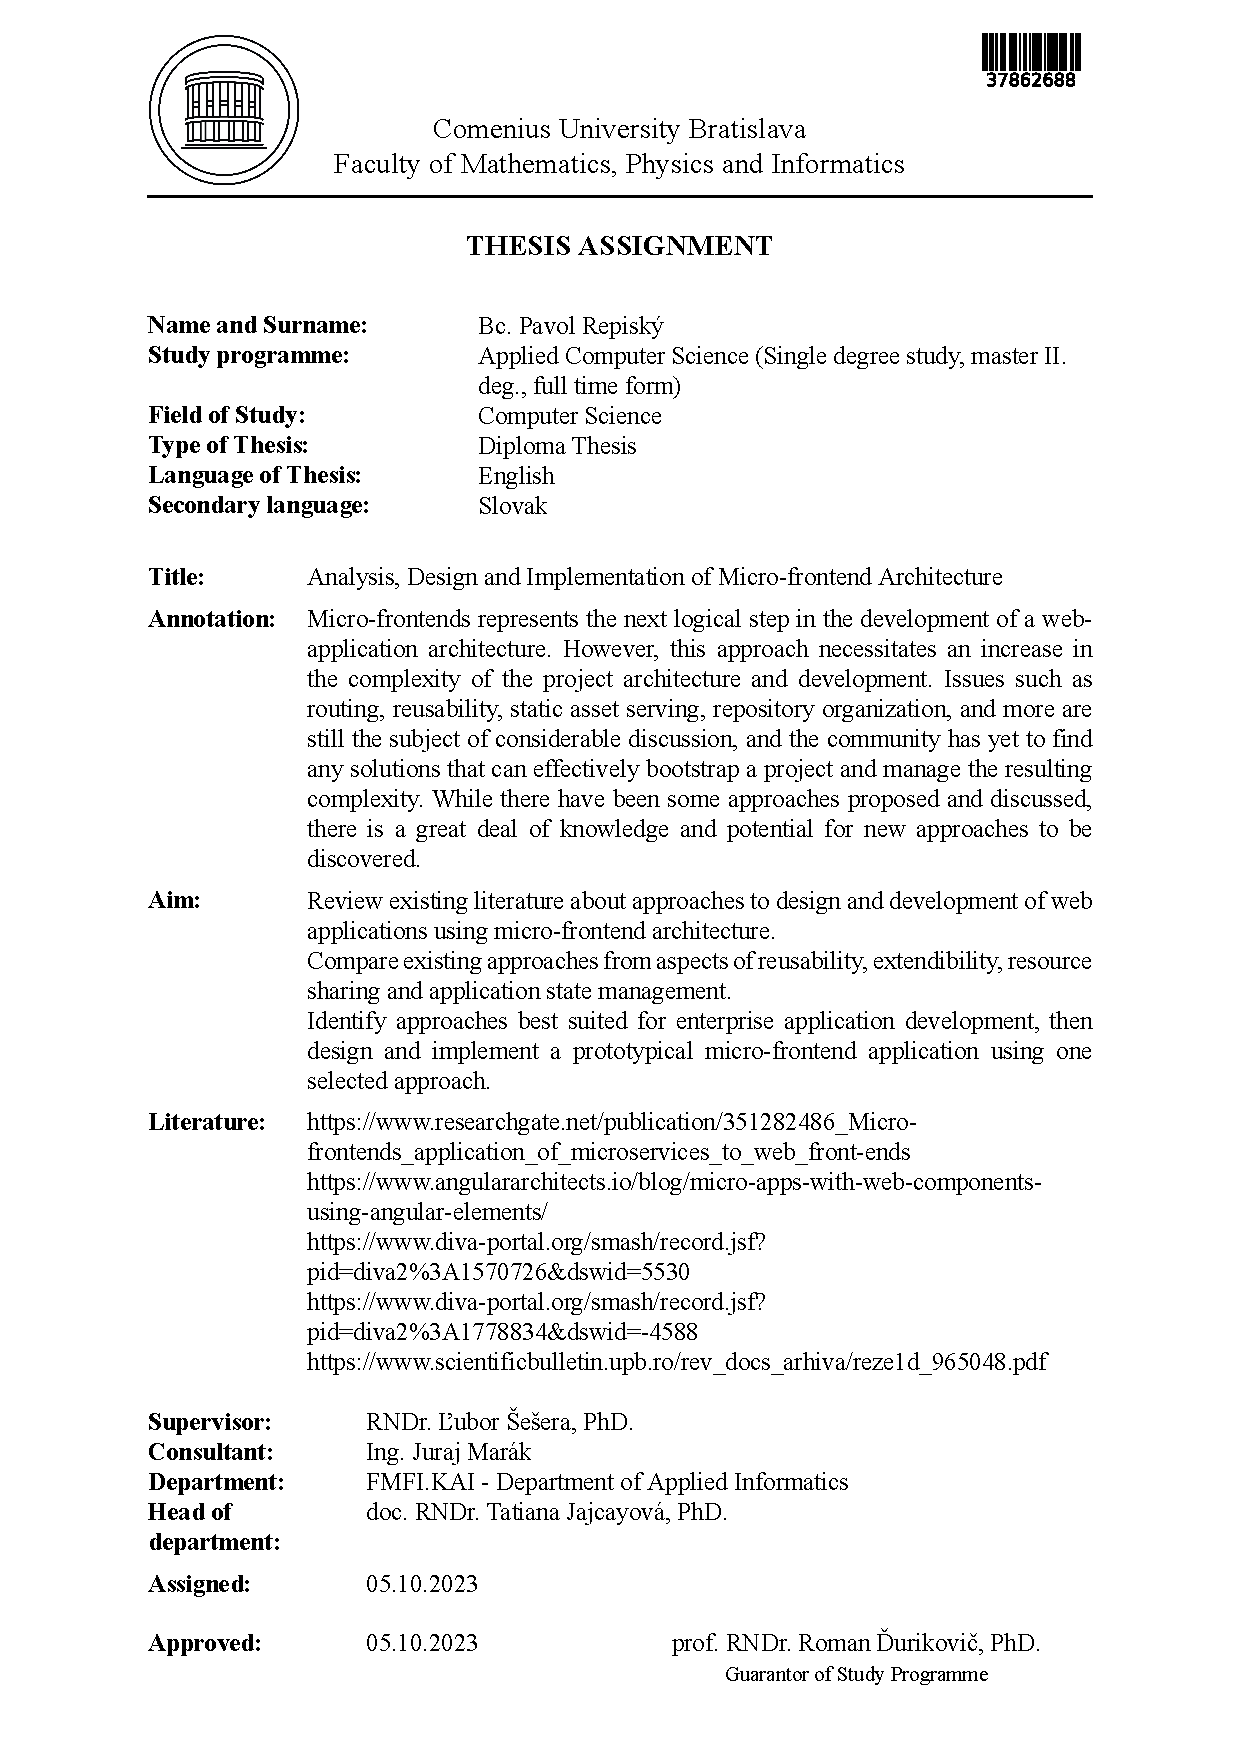
\includepdf{images/zadanie-en.pdf}
% --- Koniec zadania


% -------------------
%   Poďakovanie - nepovinné
% -------------------
\newpage
\thispagestyle{empty}
\chapter*{Acknowledgement}\label{chap:thank_you}
Tu môžete poďakovať školiteľovi, prípadne
ďalším osobám, ktoré vám s prácou nejako pomohli, poradili,
poskytli dáta a podobne.

\vfill\eject 
% --- Koniec poďakovania

% -------------------
%   Abstrakt - Slovensky
% -------------------

\newpage 
\thispagestyle{empty}
\chapter*{Abstrakt}\label{chap:abstract_sk}
Slovenský abstrakt v rozsahu 100-500 slov, jeden odstavec. Abstrakt
stručne sumarizuje výsledky práce. Mal by byť pochopiteľný pre bežného
informatika. Nemal by teda využívať skratky, termíny alebo označenie
zavedené v práci, okrem tých, ktoré sú všeobecne známe.

\paragraph*{Kľúčové slová:} jedno, druhé, tretie (prípadne štvrté, piate)
% --- Koniec Abstrakt - Slovensky


% -------------------
% --- Abstrakt - Anglicky 
% -------------------
\newpage 
\thispagestyle{empty}
\chapter*{Abstract}\label{chap:abstract_en}
Abstract in the English language (translation of the abstract in the
Slovak language).

\paragraph*{Keywords:} 
% --- Koniec Abstrakt - Anglicky

% -------------------
% --- Predhovor - v informatike sa zvacsa nepouziva
% -------------------
%\newpage 
%
%
%\chapter*{Preface} %
%
%Predhovor je všeobecná informácia o práci, obsahuje hlavnú charakteristiku práce 
%a okolnosti jej vzniku. Autor zdôvodní výber témy, stručne informuje o cieľoch 
%a význame práce, spomenie domáci a zahraničný kontext, komu je práca určená, 
%použité metódy, stav poznania; autor stručne charakterizuje svoj prístup a svoje
%hľadisko. 
%
% --- Koniec Predhovor


% -------------------
% --- Obsah
% -------------------

\newpage 

\tableofcontents

% ---  Koniec Obsahu

% -------------------
% --- Zoznamy tabuliek, obrázkov - nepovinne
% -------------------

\newpage 

\listoffigures
\listoftables

% ---  Koniec Zoznamov

\mainmatter
\pagestyle{headings}

\input chapters/Introduction/Introduction.tex 
\input chapters/LiteratureReview.tex
\input chapters/Analysis/Main.tex
\input chapters/Design.tex
\input chapters/Implementation.tex
\input chapters/Conclusion.tex

%\input zaver.tex

% -------------------
% --- Bibliografia
% -------------------


\newpage	

\backmatter

\thispagestyle{empty}
\clearpage

\bibliographystyle{plain}
\bibliography{literatura} 

%Prípadne môžete napísať literatúru priamo tu
%\begin{thebibliography}{5}
 
%\bibitem{br1} MOLINA H. G. - ULLMAN J. D. - WIDOM J., 2002, Database Systems, Upper Saddle River : Prentice-Hall, 2002, 1119 s., Pearson International edition, 0-13-098043-9

%\bibitem{br2} MOLINA H. G. - ULLMAN J. D. - WIDOM J., 2000 , Databasse System implementation, New Jersey : Prentice-Hall, 2000, 653s., ???

%\bibitem{br3} ULLMAN J. D. - WIDOM J., 1997, A First Course in Database Systems, New Jersey : Prentice-Hall, 1997, 470s., 

%\bibitem{br4} PREFUSE, 2007, The Prefuse visualization toolkit,  [online] Dostupné na internete: <http://prefuse.org/>

%\bibitem{br5} PREFUSE Forum, Sourceforge - Prefuse Forum,  [online] Dostupné na internete: <http://sourceforge.net/projects/prefuse/>

%\end{thebibliography}

%---koniec Referencii

% -------------------
%--- Prilohy---
% -------------------

%Nepovinná časť prílohy obsahuje materiály, ktoré neboli zaradené priamo  do textu. Každá príloha sa začína na novej strane.
%Zoznam príloh je súčasťou obsahu.
%
%\input appendixA.tex

%\input appendixB.tex

\end{document}






